\documentclass[1p]{elsarticle_modified}
%\bibliographystyle{elsarticle-num}

%\usepackage[colorlinks]{hyperref}
%\usepackage{abbrmath_seonhwa} %\Abb, \Ascr, \Acal ,\Abf, \Afrak
\usepackage{amsfonts}
\usepackage{amssymb}
\usepackage{amsmath}
\usepackage{amsthm}
\usepackage{scalefnt}
\usepackage{amsbsy}
\usepackage{kotex}
\usepackage{caption}
\usepackage{subfig}
\usepackage{color}
\usepackage{graphicx}
\usepackage{xcolor} %% white, black, red, green, blue, cyan, magenta, yellow
\usepackage{float}
\usepackage{setspace}
\usepackage{hyperref}

\usepackage{tikz}
\usetikzlibrary{arrows}

\usepackage{multirow}
\usepackage{array} % fixed length table
\usepackage{hhline}

%%%%%%%%%%%%%%%%%%%%%
\makeatletter
\renewcommand*\env@matrix[1][\arraystretch]{%
	\edef\arraystretch{#1}%
	\hskip -\arraycolsep
	\let\@ifnextchar\new@ifnextchar
	\array{*\c@MaxMatrixCols c}}
\makeatother %https://tex.stackexchange.com/questions/14071/how-can-i-increase-the-line-spacing-in-a-matrix
%%%%%%%%%%%%%%%

\usepackage[normalem]{ulem}

\newcommand{\msout}[1]{\ifmmode\text{\sout{\ensuremath{#1}}}\else\sout{#1}\fi}
%SOURCE: \msout is \stkout macro in https://tex.stackexchange.com/questions/20609/strikeout-in-math-mode

\newcommand{\cancel}[1]{
	\ifmmode
	{\color{red}\msout{#1}}
	\else
	{\color{red}\sout{#1}}
	\fi
}

\newcommand{\add}[1]{
	{\color{blue}\uwave{#1}}
}

\newcommand{\replace}[2]{
	\ifmmode
	{\color{red}\msout{#1}}{\color{blue}\uwave{#2}}
	\else
	{\color{red}\sout{#1}}{\color{blue}\uwave{#2}}
	\fi
}

\newcommand{\Sol}{\mathcal{S}} %segment
\newcommand{\D}{D} %diagram
\newcommand{\A}{\mathcal{A}} %arc


%%%%%%%%%%%%%%%%%%%%%%%%%%%%%5 test

\def\sl{\operatorname{\textup{SL}}(2,\Cbb)}
\def\psl{\operatorname{\textup{PSL}}(2,\Cbb)}
\def\quan{\mkern 1mu \triangleright \mkern 1mu}

\theoremstyle{definition}
\newtheorem{thm}{Theorem}[section]
\newtheorem{prop}[thm]{Proposition}
\newtheorem{lem}[thm]{Lemma}
\newtheorem{ques}[thm]{Question}
\newtheorem{cor}[thm]{Corollary}
\newtheorem{defn}[thm]{Definition}
\newtheorem{exam}[thm]{Example}
\newtheorem{rmk}[thm]{Remark}
\newtheorem{alg}[thm]{Algorithm}

\newcommand{\I}{\sqrt{-1}}
\begin{document}

%\begin{frontmatter}
%
%\title{Boundary parabolic representations of knots up to 8 crossings}
%
%%% Group authors per affiliation:
%\author{Yunhi Cho} 
%\address{Department of Mathematics, University of Seoul, Seoul, Korea}
%\ead{yhcho@uos.ac.kr}
%
%
%\author{Seonhwa Kim} %\fnref{s_kim}}
%\address{Center for Geometry and Physics, Institute for Basic Science, Pohang, 37673, Korea}
%\ead{ryeona17@ibs.re.kr}
%
%\author{Hyuk Kim}
%\address{Department of Mathematical Sciences, Seoul National University, Seoul 08826, Korea}
%\ead{hyukkim@snu.ac.kr}
%
%\author{Seokbeom Yoon}
%\address{Department of Mathematical Sciences, Seoul National University, Seoul, 08826,  Korea}
%\ead{sbyoon15@snu.ac.kr}
%
%\begin{abstract}
%We find all boundary parabolic representation of knots up to 8 crossings.
%
%\end{abstract}
%\begin{keyword}
%    \MSC[2010] 57M25 
%\end{keyword}
%
%\end{frontmatter}

%\linenumbers
%\tableofcontents
%
\newcommand\colored[1]{\textcolor{white}{\rule[-0.35ex]{0.8em}{1.4ex}}\kern-0.8em\color{red} #1}%
%\newcommand\colored[1]{\textcolor{white}{ #1}\kern-2.17ex	\textcolor{white}{ #1}\kern-1.81ex	\textcolor{white}{ #1}\kern-2.15ex\color{red}#1	}

{\Large $\underline{12n_{0177}~(K12n_{0177})}$}

\setlength{\tabcolsep}{10pt}
\renewcommand{\arraystretch}{1.6}
\vspace{1cm}\begin{tabular}{m{100pt}>{\centering\arraybackslash}m{274pt}}
\multirow{5}{120pt}{
	\centering
	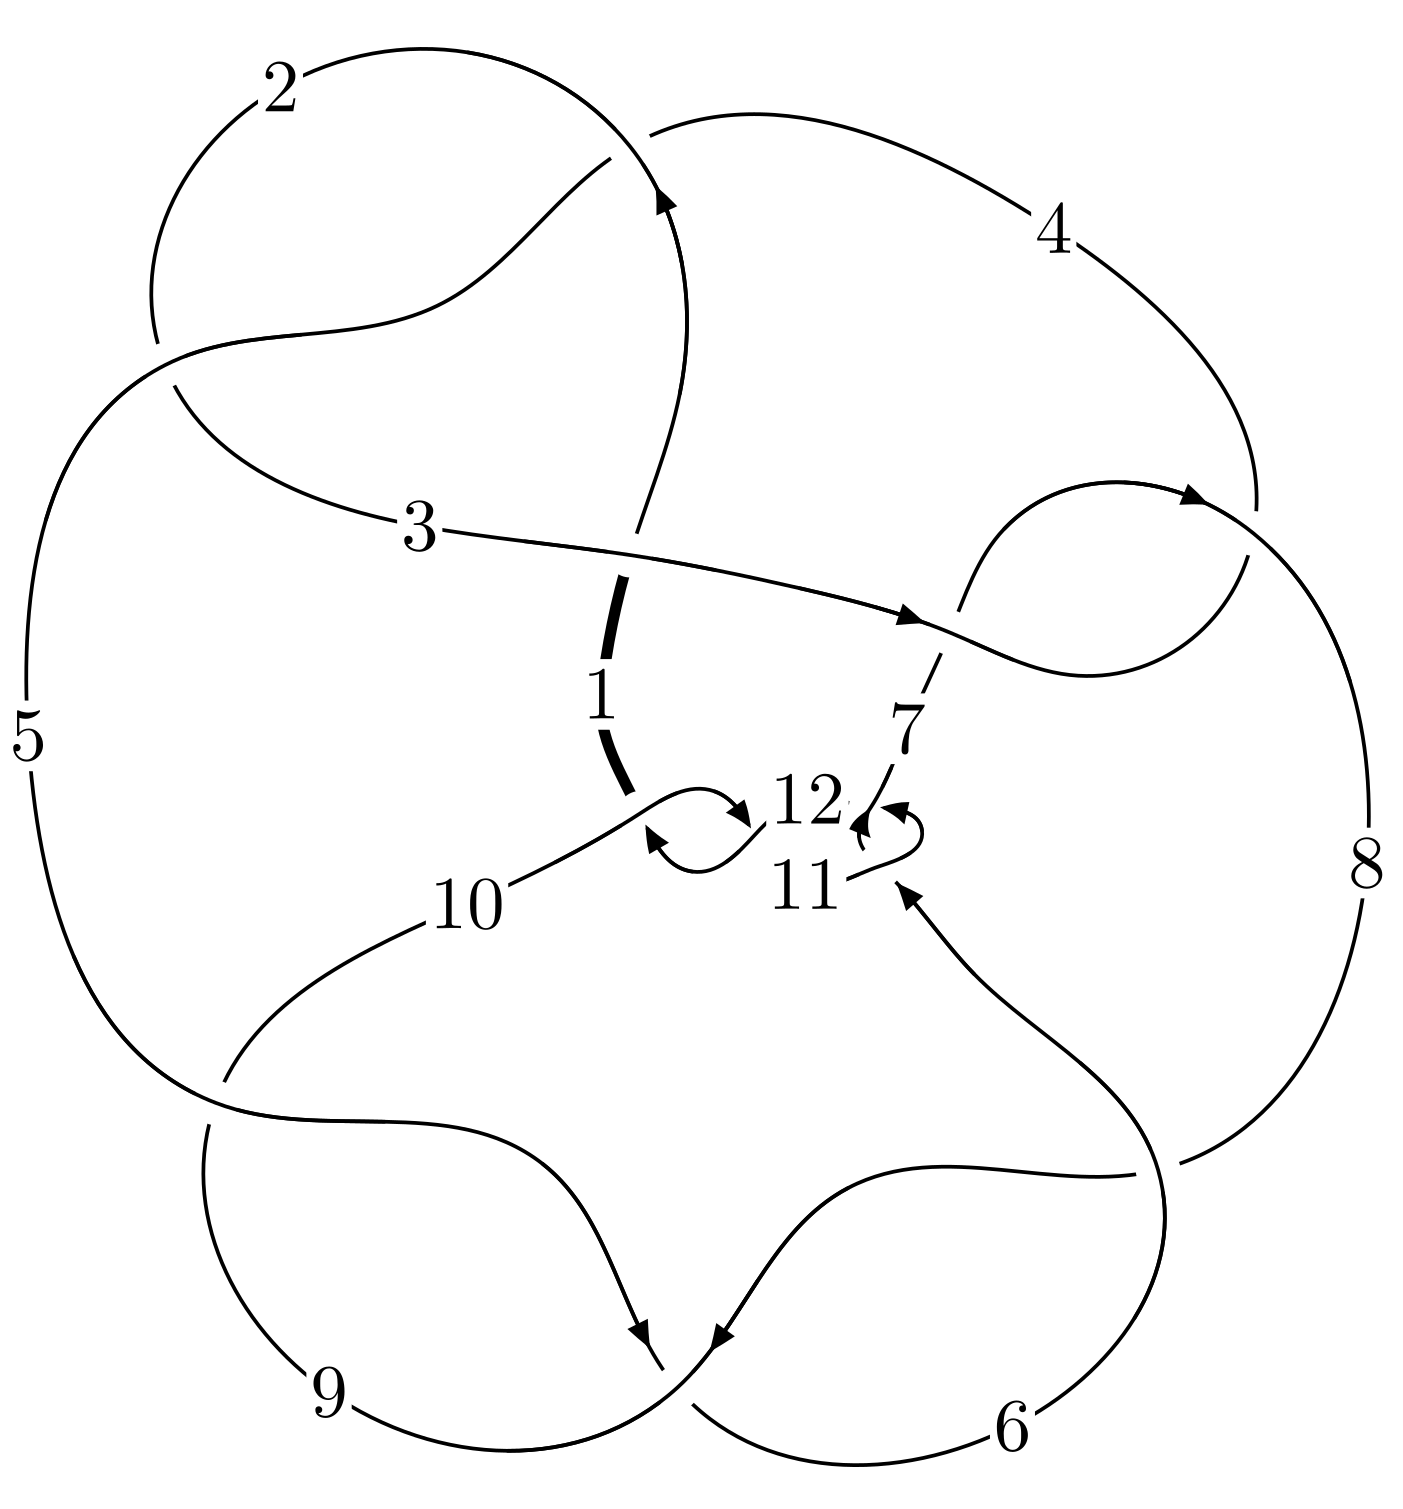
\includegraphics[width=112pt]{../../../GIT/diagram.site/Diagrams/png/2266_12n_0177.png}\\
\ \ \ A knot diagram\footnotemark}&
\allowdisplaybreaks
\textbf{Linearized knot diagam} \\
\cline{2-2}
 &
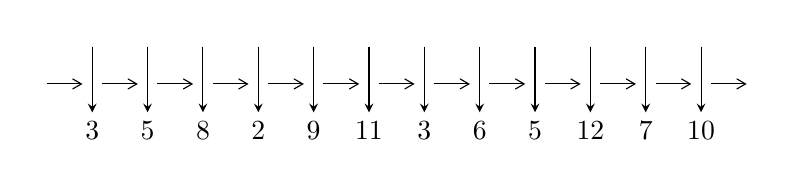
\begin{tikzpicture}[x=20pt, y=17pt]
	% nodes
	\node (C0) at (0, 0) {};
	\node (C1) at (1, 0) {};
	\node (C1U) at (1, +1) {};
	\node (C1D) at (1, -1) {3};

	\node (C2) at (2, 0) {};
	\node (C2U) at (2, +1) {};
	\node (C2D) at (2, -1) {5};

	\node (C3) at (3, 0) {};
	\node (C3U) at (3, +1) {};
	\node (C3D) at (3, -1) {8};

	\node (C4) at (4, 0) {};
	\node (C4U) at (4, +1) {};
	\node (C4D) at (4, -1) {2};

	\node (C5) at (5, 0) {};
	\node (C5U) at (5, +1) {};
	\node (C5D) at (5, -1) {9};

	\node (C6) at (6, 0) {};
	\node (C6U) at (6, +1) {};
	\node (C6D) at (6, -1) {11};

	\node (C7) at (7, 0) {};
	\node (C7U) at (7, +1) {};
	\node (C7D) at (7, -1) {3};

	\node (C8) at (8, 0) {};
	\node (C8U) at (8, +1) {};
	\node (C8D) at (8, -1) {6};

	\node (C9) at (9, 0) {};
	\node (C9U) at (9, +1) {};
	\node (C9D) at (9, -1) {5};

	\node (C10) at (10, 0) {};
	\node (C10U) at (10, +1) {};
	\node (C10D) at (10, -1) {12};

	\node (C11) at (11, 0) {};
	\node (C11U) at (11, +1) {};
	\node (C11D) at (11, -1) {7};

	\node (C12) at (12, 0) {};
	\node (C12U) at (12, +1) {};
	\node (C12D) at (12, -1) {10};
	\node (C13) at (13, 0) {};

	% arrows
	\draw[->,>={angle 60}]
	(C0) edge (C1) (C1) edge (C2) (C2) edge (C3) (C3) edge (C4) (C4) edge (C5) (C5) edge (C6) (C6) edge (C7) (C7) edge (C8) (C8) edge (C9) (C9) edge (C10) (C10) edge (C11) (C11) edge (C12) (C12) edge (C13) ;	\draw[->,>=stealth]
	(C1U) edge (C1D) (C2U) edge (C2D) (C3U) edge (C3D) (C4U) edge (C4D) (C5U) edge (C5D) (C6U) edge (C6D) (C7U) edge (C7D) (C8U) edge (C8D) (C9U) edge (C9D) (C10U) edge (C10D) (C11U) edge (C11D) (C12U) edge (C12D) ;
	\end{tikzpicture} \\
\hhline{~~} \\& 
\textbf{Solving Sequence} \\ \cline{2-2} 
 &
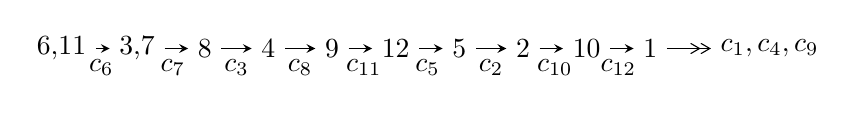
\begin{tikzpicture}[x=23pt, y=7pt]
	% node
	\node (A0) at (-1/8, 0) {6,11};
	\node (A1) at (17/16, 0) {3,7};
	\node (A2) at (17/8, 0) {8};
	\node (A3) at (25/8, 0) {4};
	\node (A4) at (33/8, 0) {9};
	\node (A5) at (41/8, 0) {12};
	\node (A6) at (49/8, 0) {5};
	\node (A7) at (57/8, 0) {2};
	\node (A8) at (65/8, 0) {10};
	\node (A9) at (73/8, 0) {1};
	\node (C1) at (1/2, -1) {$c_{6}$};
	\node (C2) at (13/8, -1) {$c_{7}$};
	\node (C3) at (21/8, -1) {$c_{3}$};
	\node (C4) at (29/8, -1) {$c_{8}$};
	\node (C5) at (37/8, -1) {$c_{11}$};
	\node (C6) at (45/8, -1) {$c_{5}$};
	\node (C7) at (53/8, -1) {$c_{2}$};
	\node (C8) at (61/8, -1) {$c_{10}$};
	\node (C9) at (69/8, -1) {$c_{12}$};
	\node (A10) at (11, 0) {$c_{1},c_{4},c_{9}$};

	% edge
	\draw[->,>=stealth]	
	(A0) edge (A1) (A1) edge (A2) (A2) edge (A3) (A3) edge (A4) (A4) edge (A5) (A5) edge (A6) (A6) edge (A7) (A7) edge (A8) (A8) edge (A9) ;
	\draw[->>,>={angle 60}]	
	(A9) edge (A10);
\end{tikzpicture} \\ 

\end{tabular} \\

\footnotetext{
The image of knot diagram is generated by the software ``\textbf{Draw programme}" developed by Andrew Bartholomew(\url{http://www.layer8.co.uk/maths/draw/index.htm\#Running-draw}), where we modified some parts for our purpose(\url{https://github.com/CATsTAILs/LinksPainter}).
}\phantom \\ \newline 
\centering \textbf{Ideals for irreducible components\footnotemark of $X_{\text{par}}$} 
 
\begin{align*}
I^u_{1}&=\langle 
5.55413\times10^{18} u^{43}-1.55873\times10^{20} u^{42}+\cdots+7.63795\times10^{20} b+1.57862\times10^{18},\\
\phantom{I^u_{1}}&\phantom{= \langle  }-5.19595\times10^{20} u^{43}-8.80516\times10^{20} u^{42}+\cdots+7.63795\times10^{20} a+1.42510\times10^{21},\;u^{44}+2 u^{43}+\cdots+u-1\rangle \\
I^u_{2}&=\langle 
u^3- u^2+b+1,\;u^4- u^2+a+2 u+1,\;u^5- u^4+u^2+u-1\rangle \\
\\
\end{align*}
\raggedright * 2 irreducible components of $\dim_{\mathbb{C}}=0$, with total 49 representations.\\
\footnotetext{All coefficients of polynomials are rational numbers. But the coefficients are sometimes approximated in decimal forms when there is not enough margin.}
\newpage
\renewcommand{\arraystretch}{1}
\centering \section*{I. $I^u_{1}= \langle 5.55\times10^{18} u^{43}-1.56\times10^{20} u^{42}+\cdots+7.64\times10^{20} b+1.58\times10^{18},\;-5.20\times10^{20} u^{43}-8.81\times10^{20} u^{42}+\cdots+7.64\times10^{20} a+1.43\times10^{21},\;u^{44}+2 u^{43}+\cdots+u-1 \rangle$}
\flushleft \textbf{(i) Arc colorings}\\
\begin{tabular}{m{7pt} m{180pt} m{7pt} m{180pt} }
\flushright $a_{6}=$&$\begin{pmatrix}1\\0\end{pmatrix}$ \\
\flushright $a_{11}=$&$\begin{pmatrix}0\\u\end{pmatrix}$ \\
\flushright $a_{3}=$&$\begin{pmatrix}0.680281 u^{43}+1.15282 u^{42}+\cdots+2.62761 u-1.86582\\-0.00727175 u^{43}+0.204078 u^{42}+\cdots+1.80199 u-0.00206682\end{pmatrix}$ \\
\flushright $a_{7}=$&$\begin{pmatrix}1\\u^2\end{pmatrix}$ \\
\flushright $a_{8}=$&$\begin{pmatrix}0.380377 u^{43}+0.278454 u^{42}+\cdots-1.47705 u+0.357193\\0.725562 u^{43}+1.09260 u^{42}+\cdots+2.20628 u-1.03029\end{pmatrix}$ \\
\flushright $a_{4}=$&$\begin{pmatrix}0.157495 u^{43}+0.219673 u^{42}+\cdots+2.88571 u-1.49128\\-0.100370 u^{43}+0.294432 u^{42}+\cdots+2.99466 u-0.234008\end{pmatrix}$ \\
\flushright $a_{9}=$&$\begin{pmatrix}-0.345186 u^{43}-0.814150 u^{42}+\cdots-3.68333 u+1.38748\\0.725562 u^{43}+1.09260 u^{42}+\cdots+2.20628 u-1.03029\end{pmatrix}$ \\
\flushright $a_{12}=$&$\begin{pmatrix}- u\\- u^3+u\end{pmatrix}$ \\
\flushright $a_{5}=$&$\begin{pmatrix}-0.727339 u^{43}-1.22924 u^{42}+\cdots+0.506371 u+1.13240\\-0.0878881 u^{43}-0.762349 u^{42}+\cdots-1.82252 u+0.614206\end{pmatrix}$ \\
\flushright $a_{2}=$&$\begin{pmatrix}0.141633 u^{43}-0.0701701 u^{42}+\cdots+2.62190 u-1.14094\\-0.0770011 u^{43}-0.0103397 u^{42}+\cdots+2.58613 u-0.141084\end{pmatrix}$ \\
\flushright $a_{10}=$&$\begin{pmatrix}u^3\\u^5- u^3+u\end{pmatrix}$ \\
\flushright $a_{1}=$&$\begin{pmatrix}- u^5- u\\- u^7+u^5-2 u^3+u\end{pmatrix}$\\&\end{tabular}
\flushleft \textbf{(ii) Obstruction class $= -1$}\\~\\
\flushleft \textbf{(iii) Cusp Shapes $= \frac{2222195580300966085542}{763794622492335702017} u^{43}+\frac{3198001597405456212425}{763794622492335702017} u^{42}+\cdots-\frac{5752714676140583930170}{763794622492335702017} u-\frac{8762178869972642405852}{763794622492335702017}$}\\~\\
\newpage\renewcommand{\arraystretch}{1}
\flushleft \textbf{(iv) u-Polynomials at the component}\newline \\
\begin{tabular}{m{50pt}|m{274pt}}
Crossings & \hspace{64pt}u-Polynomials at each crossing \\
\hline $$\begin{aligned}c_{1}\end{aligned}$$&$\begin{aligned}
&u^{44}+46 u^{43}+\cdots+113 u+1
\end{aligned}$\\
\hline $$\begin{aligned}c_{2},c_{4}\end{aligned}$$&$\begin{aligned}
&u^{44}-6 u^{43}+\cdots- u-1
\end{aligned}$\\
\hline $$\begin{aligned}c_{3},c_{7}\end{aligned}$$&$\begin{aligned}
&u^{44}- u^{43}+\cdots+416 u+32
\end{aligned}$\\
\hline $$\begin{aligned}c_{5},c_{8},c_{9}\end{aligned}$$&$\begin{aligned}
&u^{44}-2 u^{43}+\cdots- u-1
\end{aligned}$\\
\hline $$\begin{aligned}c_{6},c_{11}\end{aligned}$$&$\begin{aligned}
&u^{44}-2 u^{43}+\cdots- u-1
\end{aligned}$\\
\hline $$\begin{aligned}c_{10},c_{12}\end{aligned}$$&$\begin{aligned}
&u^{44}+18 u^{43}+\cdots+7 u+1
\end{aligned}$\\
\hline
\end{tabular}\\~\\
\newpage\renewcommand{\arraystretch}{1}
\flushleft \textbf{(v) Riley Polynomials at the component}\newline \\
\begin{tabular}{m{50pt}|m{274pt}}
Crossings & \hspace{64pt}Riley Polynomials at each crossing \\
\hline $$\begin{aligned}c_{1}\end{aligned}$$&$\begin{aligned}
&y^{44}-90 y^{43}+\cdots-1337 y+1
\end{aligned}$\\
\hline $$\begin{aligned}c_{2},c_{4}\end{aligned}$$&$\begin{aligned}
&y^{44}-46 y^{43}+\cdots-113 y+1
\end{aligned}$\\
\hline $$\begin{aligned}c_{3},c_{7}\end{aligned}$$&$\begin{aligned}
&y^{44}-33 y^{43}+\cdots-42496 y+1024
\end{aligned}$\\
\hline $$\begin{aligned}c_{5},c_{8},c_{9}\end{aligned}$$&$\begin{aligned}
&y^{44}+30 y^{43}+\cdots-7 y+1
\end{aligned}$\\
\hline $$\begin{aligned}c_{6},c_{11}\end{aligned}$$&$\begin{aligned}
&y^{44}-18 y^{43}+\cdots-7 y+1
\end{aligned}$\\
\hline $$\begin{aligned}c_{10},c_{12}\end{aligned}$$&$\begin{aligned}
&y^{44}+18 y^{43}+\cdots-7 y+1
\end{aligned}$\\
\hline
\end{tabular}\\~\\
\newpage\flushleft \textbf{(vi) Complex Volumes and Cusp Shapes}
$$\begin{array}{c|c|c}  
\text{Solutions to }I^u_{1}& \I (\text{vol} + \sqrt{-1}CS) & \text{Cusp shape}\\
 \hline 
\begin{aligned}
u &= -0.932256 + 0.333118 I \\
a &= \phantom{-}2.11928 + 0.73637 I \\
b &= \phantom{-}1.213880 + 0.113209 I\end{aligned}
 & -3.19612 + 1.16436 I & -18.0367 - 4.2407 I \\ \hline\begin{aligned}
u &= -0.932256 - 0.333118 I \\
a &= \phantom{-}2.11928 - 0.73637 I \\
b &= \phantom{-}1.213880 - 0.113209 I\end{aligned}
 & -3.19612 - 1.16436 I & -18.0367 + 4.2407 I \\ \hline\begin{aligned}
u &= -0.811966 + 0.606824 I \\
a &= -0.214198 - 0.517770 I \\
b &= -0.639085 - 0.323465 I\end{aligned}
 & \phantom{-}1.69246 + 2.33995 I & -6.03512 - 4.58901 I \\ \hline\begin{aligned}
u &= -0.811966 - 0.606824 I \\
a &= -0.214198 + 0.517770 I \\
b &= -0.639085 + 0.323465 I\end{aligned}
 & \phantom{-}1.69246 - 2.33995 I & -6.03512 + 4.58901 I \\ \hline\begin{aligned}
u &= \phantom{-}0.832515 + 0.488298 I \\
a &= -8.47385 - 3.13565 I \\
b &= -1.08225 - 8.34772 I\end{aligned}
 & \phantom{-}0.05907 - 2.03841 I & -80.5474 - 19.3778 I \\ \hline\begin{aligned}
u &= \phantom{-}0.832515 - 0.488298 I \\
a &= -8.47385 + 3.13565 I \\
b &= -1.08225 + 8.34772 I\end{aligned}
 & \phantom{-}0.05907 + 2.03841 I & -80.5474 + 19.3778 I \\ \hline\begin{aligned}
u &= -0.462434 + 0.927925 I \\
a &= \phantom{-}0.0471309 + 0.1087380 I \\
b &= \phantom{-}1.40403 + 0.74743 I\end{aligned}
 & -2.93440 - 8.69141 I & -10.66822 + 4.32970 I \\ \hline\begin{aligned}
u &= -0.462434 - 0.927925 I \\
a &= \phantom{-}0.0471309 - 0.1087380 I \\
b &= \phantom{-}1.40403 - 0.74743 I\end{aligned}
 & -2.93440 + 8.69141 I & -10.66822 - 4.32970 I \\ \hline\begin{aligned}
u &= \phantom{-}0.934426 + 0.187999 I \\
a &= -2.13830 + 1.36144 I \\
b &= -0.759161 + 0.468019 I\end{aligned}
 & -1.48992 + 2.07213 I & -15.1717 - 3.4409 I \\ \hline\begin{aligned}
u &= \phantom{-}0.934426 - 0.187999 I \\
a &= -2.13830 - 1.36144 I \\
b &= -0.759161 - 0.468019 I\end{aligned}
 & -1.48992 - 2.07213 I & -15.1717 + 3.4409 I\\
 \hline 
 \end{array}$$\newpage$$\begin{array}{c|c|c}  
\text{Solutions to }I^u_{1}& \I (\text{vol} + \sqrt{-1}CS) & \text{Cusp shape}\\
 \hline 
\begin{aligned}
u &= \phantom{-}0.482142 + 0.949428 I \\
a &= -0.0877578 - 0.0008070 I \\
b &= -1.354460 + 0.278382 I\end{aligned}
 & -6.98988 + 2.57441 I & -14.1642 - 0.9556 I \\ \hline\begin{aligned}
u &= \phantom{-}0.482142 - 0.949428 I \\
a &= -0.0877578 + 0.0008070 I \\
b &= -1.354460 - 0.278382 I\end{aligned}
 & -6.98988 - 2.57441 I & -14.1642 + 0.9556 I \\ \hline\begin{aligned}
u &= -0.996393 + 0.394966 I \\
a &= \phantom{-}1.48606 - 0.29444 I \\
b &= \phantom{-}0.886377 + 0.223778 I\end{aligned}
 & -3.65397 + 1.39656 I & -17.3361 - 0.7595 I \\ \hline\begin{aligned}
u &= -0.996393 - 0.394966 I \\
a &= \phantom{-}1.48606 + 0.29444 I \\
b &= \phantom{-}0.886377 - 0.223778 I\end{aligned}
 & -3.65397 - 1.39656 I & -17.3361 + 0.7595 I \\ \hline\begin{aligned}
u &= -0.940835 + 0.551460 I \\
a &= -0.76026 - 1.52020 I \\
b &= -1.52495 - 0.13898 I\end{aligned}
 & \phantom{-}1.36697 + 2.08215 I & -9.41465 - 2.27806 I \\ \hline\begin{aligned}
u &= -0.940835 - 0.551460 I \\
a &= -0.76026 + 1.52020 I \\
b &= -1.52495 + 0.13898 I\end{aligned}
 & \phantom{-}1.36697 - 2.08215 I & -9.41465 + 2.27806 I \\ \hline\begin{aligned}
u &= -0.519753 + 0.965172 I \\
a &= \phantom{-}0.0449987 - 0.1105440 I \\
b &= \phantom{-}1.073030 - 0.166548 I\end{aligned}
 & -2.51155 + 3.63795 I & -12.71077 - 3.32802 I \\ \hline\begin{aligned}
u &= -0.519753 - 0.965172 I \\
a &= \phantom{-}0.0449987 + 0.1105440 I \\
b &= \phantom{-}1.073030 + 0.166548 I\end{aligned}
 & -2.51155 - 3.63795 I & -12.71077 + 3.32802 I \\ \hline\begin{aligned}
u &= \phantom{-}1.025600 + 0.460789 I \\
a &= -0.04638 - 1.42837 I \\
b &= \phantom{-}0.097152 + 0.226092 I\end{aligned}
 & -3.18176 - 4.85577 I & -16.2664 + 7.5137 I \\ \hline\begin{aligned}
u &= \phantom{-}1.025600 - 0.460789 I \\
a &= -0.04638 + 1.42837 I \\
b &= \phantom{-}0.097152 - 0.226092 I\end{aligned}
 & -3.18176 + 4.85577 I & -16.2664 - 7.5137 I\\
 \hline 
 \end{array}$$\newpage$$\begin{array}{c|c|c}  
\text{Solutions to }I^u_{1}& \I (\text{vol} + \sqrt{-1}CS) & \text{Cusp shape}\\
 \hline 
\begin{aligned}
u &= \phantom{-}1.005340 + 0.543119 I \\
a &= \phantom{-}1.45241 - 1.16375 I \\
b &= \phantom{-}1.010000 + 0.655687 I\end{aligned}
 & -1.71867 - 4.49690 I & -15.4552 + 5.1685 I \\ \hline\begin{aligned}
u &= \phantom{-}1.005340 - 0.543119 I \\
a &= \phantom{-}1.45241 + 1.16375 I \\
b &= \phantom{-}1.010000 - 0.655687 I\end{aligned}
 & -1.71867 + 4.49690 I & -15.4552 - 5.1685 I \\ \hline\begin{aligned}
u &= -1.042980 + 0.576491 I \\
a &= -2.06544 - 1.02569 I \\
b &= -1.108870 + 0.723364 I\end{aligned}
 & \phantom{-}0.96122 + 8.18685 I & -10.86677 - 8.84051 I \\ \hline\begin{aligned}
u &= -1.042980 - 0.576491 I \\
a &= -2.06544 + 1.02569 I \\
b &= -1.108870 - 0.723364 I\end{aligned}
 & \phantom{-}0.96122 - 8.18685 I & -10.86677 + 8.84051 I \\ \hline\begin{aligned}
u &= -0.484164 + 0.645863 I \\
a &= -0.335926 + 0.386406 I \\
b &= -0.946963 - 0.737557 I\end{aligned}
 & \phantom{-}2.57983 - 3.38804 I & -7.14865 + 3.85146 I \\ \hline\begin{aligned}
u &= -0.484164 - 0.645863 I \\
a &= -0.335926 - 0.386406 I \\
b &= -0.946963 + 0.737557 I\end{aligned}
 & \phantom{-}2.57983 + 3.38804 I & -7.14865 - 3.85146 I \\ \hline\begin{aligned}
u &= \phantom{-}0.572656 + 0.492792 I \\
a &= -0.479357 + 0.261809 I \\
b &= \phantom{-}0.622384 - 0.489340 I\end{aligned}
 & -0.415071 + 0.135386 I & -12.51812 - 0.53462 I \\ \hline\begin{aligned}
u &= \phantom{-}0.572656 - 0.492792 I \\
a &= -0.479357 - 0.261809 I \\
b &= \phantom{-}0.622384 + 0.489340 I\end{aligned}
 & -0.415071 - 0.135386 I & -12.51812 + 0.53462 I \\ \hline\begin{aligned}
u &= \phantom{-}1.272740 + 0.019314 I \\
a &= \phantom{-}1.88935 - 0.59100 I \\
b &= \phantom{-}1.50663 - 0.34571 I\end{aligned}
 & -9.39659 + 6.06487 I & -16.0679 - 3.3672 I \\ \hline\begin{aligned}
u &= \phantom{-}1.272740 - 0.019314 I \\
a &= \phantom{-}1.88935 + 0.59100 I \\
b &= \phantom{-}1.50663 + 0.34571 I\end{aligned}
 & -9.39659 - 6.06487 I & -16.0679 + 3.3672 I\\
 \hline 
 \end{array}$$\newpage$$\begin{array}{c|c|c}  
\text{Solutions to }I^u_{1}& \I (\text{vol} + \sqrt{-1}CS) & \text{Cusp shape}\\
 \hline 
\begin{aligned}
u &= -1.27574\phantom{ +0.000000I} \\
a &= -2.04286\phantom{ +0.000000I} \\
b &= -1.59279\phantom{ +0.000000I}\end{aligned}
 & -13.6601\phantom{ +0.000000I} & -18.7020\phantom{ +0.000000I} \\ \hline\begin{aligned}
u &= \phantom{-}0.928890 + 0.877784 I \\
a &= \phantom{-}0.288927 + 0.058403 I \\
b &= -0.0255637 - 0.0518981 I\end{aligned}
 & \phantom{-}9.64608 - 3.25423 I & \phantom{-}3.42401 + 0. I\phantom{ +0.000000I} \\ \hline\begin{aligned}
u &= \phantom{-}0.928890 - 0.877784 I \\
a &= \phantom{-}0.288927 - 0.058403 I \\
b &= -0.0255637 + 0.0518981 I\end{aligned}
 & \phantom{-}9.64608 + 3.25423 I & \phantom{-}3.42401 + 0. I\phantom{ +0.000000I} \\ \hline\begin{aligned}
u &= -1.140930 + 0.668019 I \\
a &= \phantom{-}1.78965 + 0.99216 I \\
b &= \phantom{-}1.58220 - 0.85694 I\end{aligned}
 & -5.0177 + 14.5388 I & -12.0000 - 8.1006 I \\ \hline\begin{aligned}
u &= -1.140930 - 0.668019 I \\
a &= \phantom{-}1.78965 - 0.99216 I \\
b &= \phantom{-}1.58220 + 0.85694 I\end{aligned}
 & -5.0177 - 14.5388 I & -12.0000 + 8.1006 I \\ \hline\begin{aligned}
u &= \phantom{-}1.147110 + 0.679799 I \\
a &= -1.30957 + 1.19970 I \\
b &= -1.45466 - 0.44146 I\end{aligned}
 & -9.05324 - 8.53642 I & -12.00000 + 5.03243 I \\ \hline\begin{aligned}
u &= \phantom{-}1.147110 - 0.679799 I \\
a &= -1.30957 - 1.19970 I \\
b &= -1.45466 + 0.44146 I\end{aligned}
 & -9.05324 + 8.53642 I & -12.00000 - 5.03243 I \\ \hline\begin{aligned}
u &= -0.454054 + 0.487305 I \\
a &= -0.035389 - 0.728908 I \\
b &= -0.876425 + 0.512471 I\end{aligned}
 & \phantom{-}2.46066 + 2.02868 I & -5.66385 - 3.37535 I \\ \hline\begin{aligned}
u &= -0.454054 - 0.487305 I \\
a &= -0.035389 + 0.728908 I \\
b &= -0.876425 - 0.512471 I\end{aligned}
 & \phantom{-}2.46066 - 2.02868 I & -5.66385 + 3.37535 I \\ \hline\begin{aligned}
u &= -1.152990 + 0.700059 I \\
a &= \phantom{-}0.682516 + 1.130440 I \\
b &= \phantom{-}1.087850 - 0.088161 I\end{aligned}
 & -4.49244 + 2.47578 I & -12.00000 + 0. I\phantom{ +0.000000I}\\
 \hline 
 \end{array}$$\newpage$$\begin{array}{c|c|c}  
\text{Solutions to }I^u_{1}& \I (\text{vol} + \sqrt{-1}CS) & \text{Cusp shape}\\
 \hline 
\begin{aligned}
u &= -1.152990 - 0.700059 I \\
a &= \phantom{-}0.682516 - 1.130440 I \\
b &= \phantom{-}1.087850 + 0.088161 I\end{aligned}
 & -4.49244 - 2.47578 I & -12.00000 + 0. I\phantom{ +0.000000I} \\ \hline\begin{aligned}
u &= \phantom{-}0.435796\phantom{ +0.000000I} \\
a &= -0.661080\phantom{ +0.000000I} \\
b &= \phantom{-}0.319506\phantom{ +0.000000I}\end{aligned}
 & -0.646256\phantom{ +0.000000I} & -15.3650\phantom{ +0.000000I} \\ \hline\begin{aligned}
u &= \phantom{-}0.157314 + 0.396862 I \\
a &= -0.50192 + 2.61945 I \\
b &= \phantom{-}0.425511 + 0.468538 I\end{aligned}
 & -1.15253 + 1.27543 I & -10.53847 - 1.56080 I \\ \hline\begin{aligned}
u &= \phantom{-}0.157314 - 0.396862 I \\
a &= -0.50192 - 2.61945 I \\
b &= \phantom{-}0.425511 - 0.468538 I\end{aligned}
 & -1.15253 - 1.27543 I & -10.53847 + 1.56080 I\\
 \hline 
 \end{array}$$\newpage\newpage\renewcommand{\arraystretch}{1}
\centering \section*{II. $I^u_{2}= \langle u^3- u^2+b+1,\;u^4- u^2+a+2 u+1,\;u^5- u^4+u^2+u-1 \rangle$}
\flushleft \textbf{(i) Arc colorings}\\
\begin{tabular}{m{7pt} m{180pt} m{7pt} m{180pt} }
\flushright $a_{6}=$&$\begin{pmatrix}1\\0\end{pmatrix}$ \\
\flushright $a_{11}=$&$\begin{pmatrix}0\\u\end{pmatrix}$ \\
\flushright $a_{3}=$&$\begin{pmatrix}- u^4+u^2-2 u-1\\- u^3+u^2-1\end{pmatrix}$ \\
\flushright $a_{7}=$&$\begin{pmatrix}1\\u^2\end{pmatrix}$ \\
\flushright $a_{8}=$&$\begin{pmatrix}1\\u^2\end{pmatrix}$ \\
\flushright $a_{4}=$&$\begin{pmatrix}- u^4+u^2-2 u-1\\- u^3+u^2-1\end{pmatrix}$ \\
\flushright $a_{9}=$&$\begin{pmatrix}- u^2+1\\u^2\end{pmatrix}$ \\
\flushright $a_{12}=$&$\begin{pmatrix}- u\\- u^3+u\end{pmatrix}$ \\
\flushright $a_{5}=$&$\begin{pmatrix}u^4- u^2+1\\- u^4\end{pmatrix}$ \\
\flushright $a_{2}=$&$\begin{pmatrix}-2 u^4+2 u^2-2 u-2\\u^4- u^3+u^2-1\end{pmatrix}$ \\
\flushright $a_{10}=$&$\begin{pmatrix}u^3\\u^4- u^3- u^2+1\end{pmatrix}$ \\
\flushright $a_{1}=$&$\begin{pmatrix}- u^4+u^2-1\\u^4\end{pmatrix}$\\&\end{tabular}
\flushleft \textbf{(ii) Obstruction class $= 1$}\\~\\
\flushleft \textbf{(iii) Cusp Shapes $= u^4- u^3+6 u^2-4 u-15$}\\~\\
\newpage\renewcommand{\arraystretch}{1}
\flushleft \textbf{(iv) u-Polynomials at the component}\newline \\
\begin{tabular}{m{50pt}|m{274pt}}
Crossings & \hspace{64pt}u-Polynomials at each crossing \\
\hline $$\begin{aligned}c_{1},c_{2}\end{aligned}$$&$\begin{aligned}
&(u-1)^5
\end{aligned}$\\
\hline $$\begin{aligned}c_{3},c_{7}\end{aligned}$$&$\begin{aligned}
&u^5
\end{aligned}$\\
\hline $$\begin{aligned}c_{4}\end{aligned}$$&$\begin{aligned}
&(u+1)^5
\end{aligned}$\\
\hline $$\begin{aligned}c_{5},c_{10}\end{aligned}$$&$\begin{aligned}
&u^5- u^4+4 u^3-3 u^2+3 u-1
\end{aligned}$\\
\hline $$\begin{aligned}c_{6}\end{aligned}$$&$\begin{aligned}
&u^5- u^4+u^2+u-1
\end{aligned}$\\
\hline $$\begin{aligned}c_{8},c_{9},c_{12}\end{aligned}$$&$\begin{aligned}
&u^5+u^4+4 u^3+3 u^2+3 u+1
\end{aligned}$\\
\hline $$\begin{aligned}c_{11}\end{aligned}$$&$\begin{aligned}
&u^5+u^4- u^2+u+1
\end{aligned}$\\
\hline
\end{tabular}\\~\\
\newpage\renewcommand{\arraystretch}{1}
\flushleft \textbf{(v) Riley Polynomials at the component}\newline \\
\begin{tabular}{m{50pt}|m{274pt}}
Crossings & \hspace{64pt}Riley Polynomials at each crossing \\
\hline $$\begin{aligned}c_{1},c_{2},c_{4}\end{aligned}$$&$\begin{aligned}
&(y-1)^5
\end{aligned}$\\
\hline $$\begin{aligned}c_{3},c_{7}\end{aligned}$$&$\begin{aligned}
&y^5
\end{aligned}$\\
\hline $$\begin{aligned}c_{5},c_{8},c_{9}\\c_{10},c_{12}\end{aligned}$$&$\begin{aligned}
&y^5+7 y^4+16 y^3+13 y^2+3 y-1
\end{aligned}$\\
\hline $$\begin{aligned}c_{6},c_{11}\end{aligned}$$&$\begin{aligned}
&y^5- y^4+4 y^3-3 y^2+3 y-1
\end{aligned}$\\
\hline
\end{tabular}\\~\\
\newpage\flushleft \textbf{(vi) Complex Volumes and Cusp Shapes}
$$\begin{array}{c|c|c}  
\text{Solutions to }I^u_{2}& \I (\text{vol} + \sqrt{-1}CS) & \text{Cusp shape}\\
 \hline 
\begin{aligned}
u &= -0.758138 + 0.584034 I \\
a &= \phantom{-}1.47956 - 1.63976 I \\
b &= -1.10636 - 1.69341 I\end{aligned}
 & \phantom{-}0.17487 + 2.21397 I & -11.6350 - 8.8712 I \\ \hline\begin{aligned}
u &= -0.758138 - 0.584034 I \\
a &= \phantom{-}1.47956 + 1.63976 I \\
b &= -1.10636 + 1.69341 I\end{aligned}
 & \phantom{-}0.17487 - 2.21397 I & -11.6350 + 8.8712 I \\ \hline\begin{aligned}
u &= \phantom{-}0.935538 + 0.903908 I \\
a &= \phantom{-}0.044146 - 0.313338 I \\
b &= \phantom{-}0.532511 + 0.056433 I\end{aligned}
 & \phantom{-}9.31336 - 3.33174 I & -19.7758 + 5.0940 I \\ \hline\begin{aligned}
u &= \phantom{-}0.935538 - 0.903908 I \\
a &= \phantom{-}0.044146 + 0.313338 I \\
b &= \phantom{-}0.532511 - 0.056433 I\end{aligned}
 & \phantom{-}9.31336 + 3.33174 I & -19.7758 - 5.0940 I \\ \hline\begin{aligned}
u &= \phantom{-}0.645200\phantom{ +0.000000I} \\
a &= -2.04741\phantom{ +0.000000I} \\
b &= -0.852303\phantom{ +0.000000I}\end{aligned}
 & -2.52712\phantom{ +0.000000I} & -15.1780\phantom{ +0.000000I}\\
 \hline 
 \end{array}$$\newpage
\newpage\renewcommand{\arraystretch}{1}
\centering \section*{ III. u-Polynomials}
\begin{tabular}{m{50pt}|m{274pt}}
Crossings & \hspace{64pt}u-Polynomials at each crossing \\
\hline $$\begin{aligned}c_{1}\end{aligned}$$&$\begin{aligned}
&((u-1)^5)(u^{44}+46 u^{43}+\cdots+113 u+1)
\end{aligned}$\\
\hline $$\begin{aligned}c_{2}\end{aligned}$$&$\begin{aligned}
&((u-1)^5)(u^{44}-6 u^{43}+\cdots- u-1)
\end{aligned}$\\
\hline $$\begin{aligned}c_{3},c_{7}\end{aligned}$$&$\begin{aligned}
&u^5(u^{44}- u^{43}+\cdots+416 u+32)
\end{aligned}$\\
\hline $$\begin{aligned}c_{4}\end{aligned}$$&$\begin{aligned}
&((u+1)^5)(u^{44}-6 u^{43}+\cdots- u-1)
\end{aligned}$\\
\hline $$\begin{aligned}c_{5}\end{aligned}$$&$\begin{aligned}
&(u^5- u^4+4 u^3-3 u^2+3 u-1)(u^{44}-2 u^{43}+\cdots- u-1)
\end{aligned}$\\
\hline $$\begin{aligned}c_{6}\end{aligned}$$&$\begin{aligned}
&(u^5- u^4+u^2+u-1)(u^{44}-2 u^{43}+\cdots- u-1)
\end{aligned}$\\
\hline $$\begin{aligned}c_{8},c_{9}\end{aligned}$$&$\begin{aligned}
&(u^5+u^4+4 u^3+3 u^2+3 u+1)(u^{44}-2 u^{43}+\cdots- u-1)
\end{aligned}$\\
\hline $$\begin{aligned}c_{10}\end{aligned}$$&$\begin{aligned}
&(u^5- u^4+4 u^3-3 u^2+3 u-1)(u^{44}+18 u^{43}+\cdots+7 u+1)
\end{aligned}$\\
\hline $$\begin{aligned}c_{11}\end{aligned}$$&$\begin{aligned}
&(u^5+u^4- u^2+u+1)(u^{44}-2 u^{43}+\cdots- u-1)
\end{aligned}$\\
\hline $$\begin{aligned}c_{12}\end{aligned}$$&$\begin{aligned}
&(u^5+u^4+4 u^3+3 u^2+3 u+1)(u^{44}+18 u^{43}+\cdots+7 u+1)
\end{aligned}$\\
\hline
\end{tabular}\newpage\renewcommand{\arraystretch}{1}
\centering \section*{ IV. Riley Polynomials}
\begin{tabular}{m{50pt}|m{274pt}}
Crossings & \hspace{64pt}Riley Polynomials at each crossing \\
\hline $$\begin{aligned}c_{1}\end{aligned}$$&$\begin{aligned}
&((y-1)^5)(y^{44}-90 y^{43}+\cdots-1337 y+1)
\end{aligned}$\\
\hline $$\begin{aligned}c_{2},c_{4}\end{aligned}$$&$\begin{aligned}
&((y-1)^5)(y^{44}-46 y^{43}+\cdots-113 y+1)
\end{aligned}$\\
\hline $$\begin{aligned}c_{3},c_{7}\end{aligned}$$&$\begin{aligned}
&y^5(y^{44}-33 y^{43}+\cdots-42496 y+1024)
\end{aligned}$\\
\hline $$\begin{aligned}c_{5},c_{8},c_{9}\end{aligned}$$&$\begin{aligned}
&(y^5+7 y^4+16 y^3+13 y^2+3 y-1)(y^{44}+30 y^{43}+\cdots-7 y+1)
\end{aligned}$\\
\hline $$\begin{aligned}c_{6},c_{11}\end{aligned}$$&$\begin{aligned}
&(y^5- y^4+4 y^3-3 y^2+3 y-1)(y^{44}-18 y^{43}+\cdots-7 y+1)
\end{aligned}$\\
\hline $$\begin{aligned}c_{10},c_{12}\end{aligned}$$&$\begin{aligned}
&(y^5+7 y^4+16 y^3+13 y^2+3 y-1)(y^{44}+18 y^{43}+\cdots-7 y+1)
\end{aligned}$\\
\hline
\end{tabular}
\vskip 2pc
\end{document}